\documentclass{article}

\usepackage[english]{babel}
\usepackage[utf8]{inputenc}
\usepackage{amsmath,amssymb}
\usepackage{parskip}
\usepackage{graphicx}

%code
\usepackage{listings}
\usepackage{color}
\usepackage{minted}




% Margins
\usepackage[top=2.5cm, left=3cm, right=3cm, bottom=4.0cm]{geometry}
% Colour table cells
\usepackage[table]{xcolor}

% Get larger line spacing in table
\newcommand{\tablespace}{\\[1.25mm]}
\newcommand\Tstrut{\rule{0pt}{2.6ex}}         % = `top' strut
\newcommand\tstrut{\rule{0pt}{2.0ex}}         % = `top' strut
\newcommand\Bstrut{\rule[-0.9ex]{0pt}{0pt}}   % = `bottom' strut

%%%%%%%%%%%%%%%%%
%     Title     %
%%%%%%%%%%%%%%%%%
\title{CSE344 MIDTERM PROJECT}
\author{Ümit Altıntaş \\ 171044005}
\date{\today}

\begin{document}
\maketitle
\section{DESIGN}
First of all I have created 2 shared anonymous shared memory. One of them for fridge which hold vaccines and one of them for room which citizens stay.
I have created 3 semaphore in first shared memory as classical producer consumer problem. one for put vaccine to fridge, one for take vaccine from fridge and last one for accessing fridge. Also i have created 1 semaphore in the second shared memory. This one protect  waiting citizen index. In the second shared memory there is also citizens pids.
\section{HOW TO MANAGE THEM}
when program starts I create citizen process first for accessing from other processes.
After that I create nurses and vaccinators respectively. When creation finish I  suspend main process and wait the children. When all children finish close all files, memories etc.
\section{HOW NURSE WORKS}
First nurse blocks file , read the vaccine id from file and unblock the file. When it reads ask  permission  for add vaccine to the fridge. If there enough slot in the fridge it takes the permission and increase the read vaccine id count. If it's read cause a new vaccine pair it post the vaccine semaphore for taking vaccine from fridge.
After that it prints it's status and post the fridge access semaphore. 


\section{HOW VACCINATOR WORKS}
It starts with closing unused file desriptor which is read end of pipes.
After that it ask permisson for accessing room. when it access the room first checks for is there any citizen inside. if there is not it breaks the loop and close the write part of the pipes. If there is it ask permission for accessing vaccine from fridge. when he get access  it takes the vaccine and post the buffer semaphore for nurses (which means "Hey there new slot in the buffer"). and post again fridge acces semaphore for anyone. After that he call(with writing citizens pipe)the citizen , post the room semaphore  , vaccine him and print the status. Lastly increase its vaccine count.
when vaccination finish it closes pipes.

\section{HOW CITIZEN WORKS}
It is simple process. It just wait for shot count times reading pipes. That is it.
\pagebreak


\section{SEMAPHORE}
nurses semaphore starts with buffer size.\\

fridge semaphore starts with 1.\\

vaccine semaphore starts with 0;\\

room semaphore starts with 1.\\


\section{WHAT IS WORKING WHAT IS NOT WORKING}
\subsection{WORKING}
I have testes it with 20k input and it works well now error no stuck.\\

Valgring: I have check it with valgrind and there is no error.

Sorted vaccination: In my tests it also works well since my design.

\subsection{NOT WORKING}
NOTHING! at least my tests.
\pagebreak
\section{FILE STRUCTURE}
my source files in the src folder, out files in the out folder. 
make extract outputs to the out folder.
\begin{figure}
    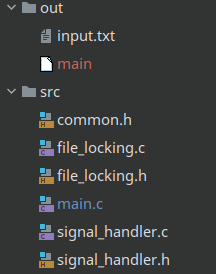
\includegraphics{files.png}
    \caption{file structure}
    \label{fig:my_label}
\end{figure}
\end{document}
